\documentclass[a4paper]{article}
\usepackage[landscape,margin=0.6cm]{geometry}
\usepackage{tikz}
\usepackage{amsmath}
\usetikzlibrary{shapes.geometric, arrows.meta, positioning, fit, backgrounds, calc, matrix}
\pagestyle{empty}

% ---------- colours ----------
\definecolor{cData}{HTML}{AED6F1}   % data nodes
\definecolor{cProc}{HTML}{ECEFF1}   % processing blocks (light gray)
\definecolor{cOff}{HTML}{B0B8BF}    % offline data generation (darker gray)
\definecolor{cMod}{HTML}{FAD7A0}    % model
\definecolor{cOpt}{HTML}{A9DFBF}    % loss / optimizer
\definecolor{cOut}{HTML}{FCF3CF}    % output artifacts

\pgfdeclarelayer{background}
\pgfsetlayers{background,main}

\newcommand{\bu}{$\bullet$\,}

\tikzset{
  blk/.style={draw, rounded corners=3pt, fill=cProc, font=\scriptsize, align=left, inner sep=3pt},
  off/.style={blk, fill=cOff, dashed, thick},
  mdl/.style={blk, fill=cMod},
  opt/.style={blk, fill=cOpt},
  dat/.style={draw, trapezium, trapezium left angle=72, trapezium right angle=108,
              fill=cData, font=\scriptsize, align=center, inner xsep=0pt, inner ysep=2pt,
              minimum height=0.8cm},
  art/.style={blk, fill=cOut, align=center, minimum width=5.0cm, minimum height=0.5cm},
  sub/.style={draw, rounded corners=2pt, fill=white, font=\scriptsize, align=left,
              text width=4.3cm, inner sep=2pt},
  ln/.style={blk, align=center, minimum width=2.3cm, minimum height=0.75cm, inner sep=2pt},
  arr/.style={-{Stealth[length=2mm,width=1.6mm]}, thick},
  darr/.style={arr, dashed},
  lbl/.style={font=\tiny\ttfamily, inner sep=1pt},
  fbox/.style={draw, rounded corners=4pt, inner sep=4pt},
  sw/.style={draw, minimum size=3mm, inner sep=0pt},
}
\newcommand{\hh}[3]{\draw[arr] (#1) -- node[lbl,above=1pt]{#3} (#2);}

\begin{document}
\centering
\scalebox{1.0}{%
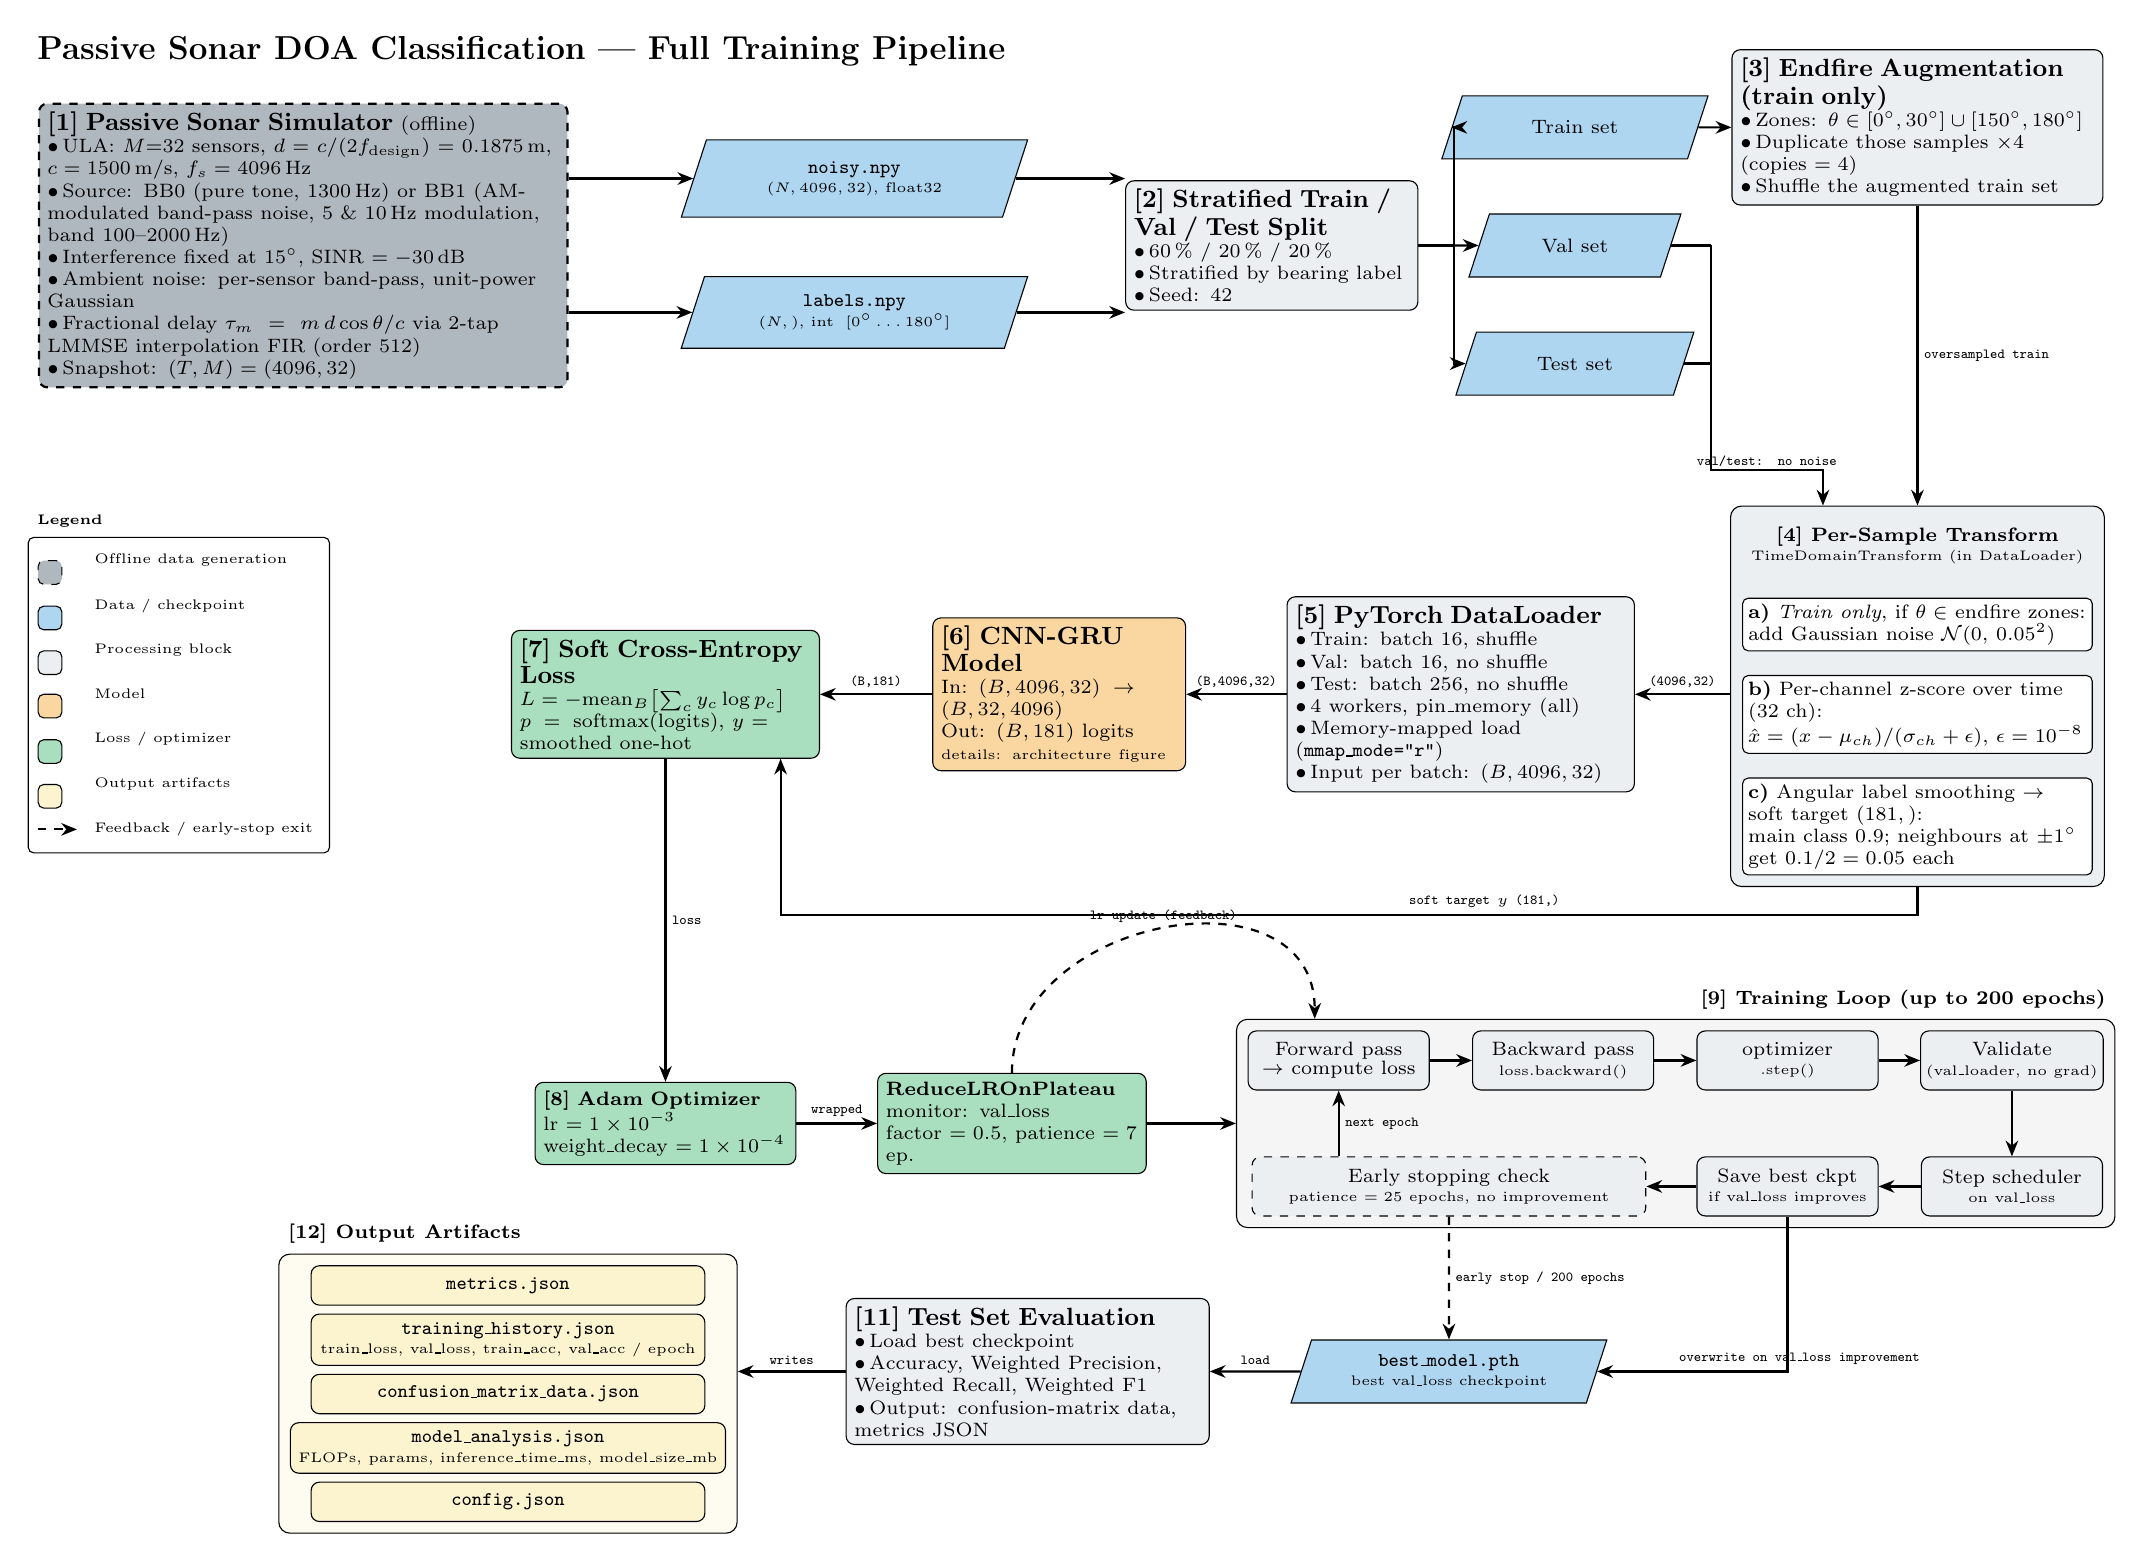
\begin{tikzpicture}

%=====================================================================
% ROW 1 (left -> right): Stage 1 -> 2
%=====================================================================
\node[off, text width=6.5cm] (sim) at (0,0) {%
  \textbf{\small [1] Passive Sonar Simulator} (offline)\\
  \bu ULA: $M{=}32$ sensors, $d=c/(2f_{\mathrm{design}})=0.1875$\,m, $c=1500$\,m/s, $f_s=4096$\,Hz\\
  \bu Source: BB0 (pure tone, 1300\,Hz) or BB1 (AM-modulated band-pass noise, 5 \& 10\,Hz modulation, band 100--2000\,Hz)\\
  \bu Interference fixed at $15^\circ$, SINR $=-30$\,dB\\
  \bu Ambient noise: per-sensor band-pass, unit-power Gaussian\\
  \bu Fractional delay $\tau_m=m\,d\cos\theta/c$ via 2-tap LMMSE interpolation FIR (order 512)\\
  \bu Snapshot: $(T,M)=(4096,32)$};

\node[dat, minimum width=4.4cm] (noisy) at (7.0,0.85)
  {\texttt{noisy.npy}\\[-1pt]{\tiny $(N,4096,32)$, float32}};
\node[dat, minimum width=4.4cm] (labs) at (7.0,-0.85)
  {\texttt{labels.npy}\\[-1pt]{\tiny $(N,)$, int \;[$0^\circ\ldots180^\circ$]}};

\node[blk, text width=3.5cm] (split) at (12.3,0) {%
  \textbf{\small [2] Stratified Train / Val / Test Split}\\
  \bu 60\,\% / 20\,\% / 20\,\%\\
  \bu Stratified by bearing label\\
  \bu Seed: 42};

\node[dat, minimum width=1.9cm] (train) at (16.15,1.5) {Train set};
\node[dat, minimum width=1.9cm] (val)   at (16.15,0)   {Val set};
\node[dat, minimum width=1.9cm] (test)  at (16.15,-1.5){Test set};

\node[blk, text width=4.5cm] (en) at (20.5,1.5) {%
  \textbf{\small [3] Endfire Augmentation (train only)}\\
  \bu Zones: $\theta\in[0^\circ,30^\circ]\cup[150^\circ,180^\circ]$\\
  \bu Duplicate those samples $\times4$ (copies $=4$)\\
  \bu Shuffle the augmented train set};

\draw[arr] (sim.east |- noisy.west) -- (noisy.west);
\draw[arr] (sim.east |- labs.west) -- (labs.west);
\draw[arr] (noisy.east) -- (noisy.east -| split.west);
\draw[arr] (labs.east) -- (labs.east -| split.west);
\draw[arr] (split.east) -- ++(0.45,0) |- (train.west);
\draw[arr] (split.east) -- (val.west);
\draw[arr] (split.east) -- ++(0.45,0) |- (test.west);
\draw[arr] (train.east) -- (en.west);

%=====================================================================
% ROW 2 (right -> left): Stages 4 -> 5 -> 6 -> 7
%=====================================================================
\node[anchor=north, font=\scriptsize\bfseries, align=center] (tt) at (20.5,-3.45)
  {[4] Per-Sample Transform\\[-1pt]{\tiny\mdseries TimeDomainTransform (in DataLoader)}};
\node[sub, below=3mm of tt] (ta)
  {\textbf{a)} \emph{Train only}, if $\theta\in$ endfire zones: add Gaussian noise $\mathcal N(0,\,0.05^2)$};
\node[sub, below=3mm of ta] (tb)
  {\textbf{b)} Per-channel z-score over time (32 ch):\\
   $\hat x=(x-\mu_{ch})/(\sigma_{ch}+\epsilon)$, $\epsilon=10^{-8}$};
\node[sub, below=3mm of tb] (tc)
  {\textbf{c)} Angular label smoothing $\to$ soft target $(181,)$:\\
   main class $0.9$; neighbours at $\pm1^\circ$ get $0.1/2=0.05$ each};

\node[blk, text width=4.2cm] (dl) at (14.7,-5.7) {%
  \textbf{\small [5] PyTorch DataLoader}\\
  \bu Train: batch 16, shuffle\\
  \bu Val: batch 16, no shuffle\\
  \bu Test: batch 256, no shuffle\\
  \bu 4 workers, pin\_memory (all)\\
  \bu Memory-mapped load (\texttt{mmap\_mode="r"})\\
  \bu Input per batch: $(B,4096,32)$};

\node[mdl, text width=3.0cm] (model) at (9.6,-5.7) {%
  \textbf{\small [6] CNN-GRU Model}\\
  In: $(B,4096,32)\to(B,32,4096)$\\
  Out: $(B,181)$ logits\\
  {\tiny details: architecture figure}};

\node[opt, text width=3.7cm] (loss) at (4.6,-5.7) {%
  \textbf{\small [7] Soft Cross-Entropy Loss}\\
  $L=-\mathrm{mean}_B\!\left[\sum_c y_c\log p_c\right]$\\
  $p=\mathrm{softmax}(\text{logits})$, $y$ = smoothed one-hot};

%=====================================================================
% ROW 3 (left -> right): Stage 8 -> Stage 9 (training loop)
%=====================================================================
\node[opt, text width=3.1cm] (adam) at (4.6,-11.15) {%
  \textbf{\scriptsize [8] Adam Optimizer}\\
  lr $=1\times10^{-3}$\\ weight\_decay $=1\times10^{-4}$};
\node[opt, text width=3.2cm] (sched) at (9.0,-11.15) {%
  \textbf{\scriptsize ReduceLROnPlateau}\\
  monitor: val\_loss\\ factor $=0.5$, patience $=7$ ep.};

% loop internals: top row L->R, bottom row R->L
\node[ln] (n1) at (13.15,-10.35) {Forward pass\\[-1pt]$\to$ compute loss};
\node[ln] (n2) at (16.0,-10.35)  {Backward pass\\[-1pt]{\tiny loss.backward()}};
\node[ln] (n3) at (18.85,-10.35) {optimizer\\[-1pt]{\tiny .step()}};
\node[ln] (n4) at (21.7,-10.35)  {Validate\\[-1pt]{\tiny (val\_loader, no grad)}};
\node[ln] (n5) at (21.7,-11.95)  {Step scheduler\\[-1pt]{\tiny on val\_loss}};
\node[ln] (n6) at (18.85,-11.95) {Save best ckpt\\[-1pt]{\tiny if val\_loss improves}};
\node[ln, dashed, minimum width=5.0cm] (n7) at (14.55,-11.95)
  {Early stopping check\\[-1pt]{\tiny patience $=25$ epochs, no improvement}};

\draw[arr] (n1) -- (n2);
\draw[arr] (n2) -- (n3);
\draw[arr] (n3) -- (n4);
\draw[arr] (n4) -- (n5);
\draw[arr] (n5) -- (n6);
\draw[arr] (n6) -- (n7);
\draw[arr] (n1.south |- n7.north) -- node[lbl,right=1pt]{next epoch} (n1.south);

%=====================================================================
% ROW 4 (right -> left): Stages 10 -> 11 -> 12
%=====================================================================
\node[dat, minimum width=4.0cm] (best) at (14.55,-14.3)
  {\texttt{best\_model.pth}\\[-1pt]{\tiny best val\_loss checkpoint}};

\node[blk, text width=4.4cm] (ev) at (9.2,-14.3) {%
  \textbf{\small [11] Test Set Evaluation}\\
  \bu Load best checkpoint\\
  \bu Accuracy, Weighted Precision, Weighted Recall, Weighted F1\\
  \bu Output: confusion-matrix data, metrics JSON};

\node[art, below=0pt] (a1) at (2.6,-12.95) {\texttt{metrics.json}};
\node[art, below=1mm of a1] (a2)
  {\texttt{training\_history.json}\\[-1pt]{\tiny train\_loss, val\_loss, train\_acc, val\_acc / epoch}};
\node[art, below=1mm of a2] (a3) {\texttt{confusion\_matrix\_data.json}};
\node[art, below=1mm of a3] (a4)
  {\texttt{model\_analysis.json}\\[-1pt]{\tiny FLOPs, params, inference\_time\_ms, model\_size\_mb}};
\node[art, below=1mm of a4] (a5) {\texttt{config.json}};

%=====================================================================
% FRAMES
%=====================================================================
\begin{pgfonlayer}{background}
  \node[fbox, fill=cProc, fit=(tt)(ta)(tb)(tc)] (tfr) {};
  \node[fbox, fill=gray!8, fit=(n1)(n2)(n3)(n4)(n5)(n6)(n7),
        label={[font=\scriptsize\bfseries, anchor=south east]north east:{[9] Training Loop (up to 200 epochs)}}] (lfr) {};
  \node[fbox, fill=cOut!30, fit=(a1)(a2)(a3)(a4)(a5),
        label={[font=\scriptsize\bfseries, anchor=south west]north west:{[12] Output Artifacts}}] (afr) {};
\end{pgfonlayer}

%=====================================================================
% ARROWS DEPENDING ON FRAMES
%=====================================================================
% train -> transform (oversampled)
\draw[arr] (en.south) -- node[lbl,right=1pt]{oversampled train} (en.south |- tfr.north);

% val / test bypass augmentation
\coordinate (jv)   at ($(val.east)+(0.5,0)$);
\coordinate (gapp) at ($(jv |- tfr.north)+(0,0.45)$);
\coordinate (jt)   at ($(tfr.north)+(-1.2,0)$);
\draw[thick] (val.east) -- (jv);
\draw[thick] (test.east) -- (test.east -| jv);
\draw[arr] (jv) -- (jv |- gapp) -- (gapp -| jt) -- (jt);
\node[lbl, above] at ($(jv |- gapp)!0.5!(gapp -| jt)$) {val/test: no noise};

% row 2
\draw[arr] (tfr.west |- dl.east) -- node[lbl,above=1pt]{(4096,32)} (dl.east);
\hh{dl.west}{model.east}{(B,4096,32)}
\hh{model.west}{loss.east}{(B,181)}

% soft target y to loss (routed under row 2)
\draw[arr] (tfr.south) -- ++(0,-0.35) -| ($(loss.south east)+(-0.5,0)$);
\node[lbl, above] at (15.0,-8.45) {soft target $y$ (181,)};

% loss -> optimizer -> scheduler -> loop
\draw[arr] (loss.south) -- node[lbl,right=1pt]{loss} (adam.north);
\draw[arr] (adam.east) -- node[lbl,above=1pt]{wrapped} (sched.west);
\draw[arr] (sched.east) -- (lfr.west |- sched.east);

% scheduler feedback (lr update) back into the loop
\draw[darr] (sched.north) to[out=90,in=90,looseness=1.3]
  node[lbl,above=1pt,pos=0.5]{lr update (feedback)} ($(lfr.north west)+(1.0,0)$);

% loop exits
\draw[darr] (n7.south) -- node[lbl,right=1pt]{early stop / 200 epochs} (best.north);
\draw[arr] (n6.south) |- (best.east);
\node[lbl, anchor=south west] at ($(best.east)+(1.0,0.05)$) {overwrite on val\_loss improvement};

% row 4
\hh{best.west}{ev.east}{load}
\draw[arr] (ev.west) -- node[lbl,above=1pt]{writes} (afr.east |- ev.west);

%=====================================================================
% TITLE + LEGEND
%=====================================================================
\node[anchor=south west, font=\large\bfseries] at (-3.5,2.15)
  {Passive Sonar DOA Classification --- Full Training Pipeline};

\matrix[draw, rounded corners=2pt, fill=white, font=\tiny, inner sep=3pt,
        row sep=2pt, column sep=3pt, anchor=north west, ampersand replacement=\&]
  (leg) at (-3.5,-3.7) {
  \node[sw, fill=cOff, dashed]{}; \& \node[anchor=west, minimum height=3mm]{Offline data generation};\\
  \node[sw, fill=cData]{};        \& \node[anchor=west, minimum height=3mm]{Data / checkpoint};\\
  \node[sw, fill=cProc]{};        \& \node[anchor=west, minimum height=3mm]{Processing block};\\
  \node[sw, fill=cMod]{};         \& \node[anchor=west, minimum height=3mm]{Model};\\
  \node[sw, fill=cOpt]{};         \& \node[anchor=west, minimum height=3mm]{Loss / optimizer};\\
  \node[sw, fill=cOut]{};         \& \node[anchor=west, minimum height=3mm]{Output artifacts};\\
  \draw[darr] (0,0) -- (0.5,0);   \& \node[anchor=west, minimum height=3mm]{Feedback / early-stop exit};\\
};
\node[font=\tiny\bfseries, anchor=south west] at (leg.north west) {Legend};

\end{tikzpicture}}
\end{document}
